\chapter{Experiências e discussão dos resultados}
\label{chap:experiencias}

Este capítulo reúne os resultados conservados nos relatórios
\path{reports/result_prediction/RESULTS.md},
\path{reports/performance/RESULTS.md},
\path{reports/rotation/RESULTS.md},
\path{reports/substitutions/RESULTS.md} e
\path{reports/horizon/RESULTS.md} do projeto \texttt{challenge-two}.
A comparação com o algoritmo genético utiliza ainda os relatórios
\path{reports/genetic_substitutions/RESULTS.md} e
\path{reports/genetic_substitutions_no_fatigue/RESULTS.md}, bem como
os respetivos ficheiros \texttt{runs.csv}.
Os valores complementares da avaliação individual e dos alinhamentos
provêm de \path{reports/performance/metrics.json}.
As experiências não foram novamente executadas para esta redação.

\section{Divisões temporais e critérios}

A Tabela~\ref{tab:divisoes} apresenta os subconjuntos utilizados. A previsão
individual exige participação e cinco jogos anteriores do jogador na
época. Para os cinco iniciais foram aceites 7\,054 jogos e excluídos
1\,229 devido a titulares ausentes ou inválidos. Por isso, as tarefas
não devem ser comparadas como se utilizassem a mesma população.

\begin{table*}[htbp]
\centering
\caption{Dimensão das divisões por tarefa.}\label{tab:divisoes}
\begin{tabular}{lrrr}
\toprule
Divisão & Jogos & Participações & Cinco inicial (jogos)\\
\midrule
Treino: 2019--20 a 2023--24 & 5\,829 & 109\,235 & 4\,600\\
Validação: 2024--25 & 1\,224 & 23\,405 & 1\,224\\
Teste: 2025--26 & 1\,230 & 23\,802 & 1\,230\\
\bottomrule
\end{tabular}
\end{table*}

A seleção usa perda logarítmica para resultados, MAE médio para produção
individual e RMSE para margem associada aos titulares. O teste é posterior
à validação e não serve para selecionar novas configurações.
O planeamento é avaliado pelo cumprimento das restrições e pelas
utilidades definidas, separadamente das métricas preditivas.

\section{Previsão de resultados}

A regressão logística com \(C=0{,}1\) obteve a menor perda de validação
entre os modelos aprendidos: 0,603, face a 0,604 nas outras configurações
logísticas, 0,612 e 0,618 no boosting e 0,614 na Random Forest.
A Tabela~\ref{tab:resultados-previsao} apresenta a avaliação final após
reajuste com treino e validação.

\begin{table*}[htbp]
\centering
\caption{Resultados de teste para previsão de vitória da equipa da casa.}
\label{tab:resultados-previsao}
\begin{tabular}{lrrrr}
\toprule
Modelo & Exatidão & Log loss & Brier & ROC-AUC\\
\midrule
Regressão logística, \(C=0{,}1\) & 0,672 & 0,603 & 0,208 & 0,729\\
Elo & 0,678 & 0,608 & 0,210 & 0,726\\
Frequência de vitória em casa & 0,554 & 0,687 & 0,247 & 0,500\\
\bottomrule
\end{tabular}
\end{table*}

A regressão logística supera a referência de frequência histórica e
apresenta erros probabilísticos ligeiramente inferiores aos do Elo.
O Elo tem maior exatidão no limiar de 0,5. Esta diferença ilustra que a
melhor classificação binária não implica a melhor qualidade probabilística.
As estimativas pontuais numa única temporada não demonstram uma diferença
estatisticamente significativa entre regressão logística e Elo.

\begin{figure*}[htbp]
\centering
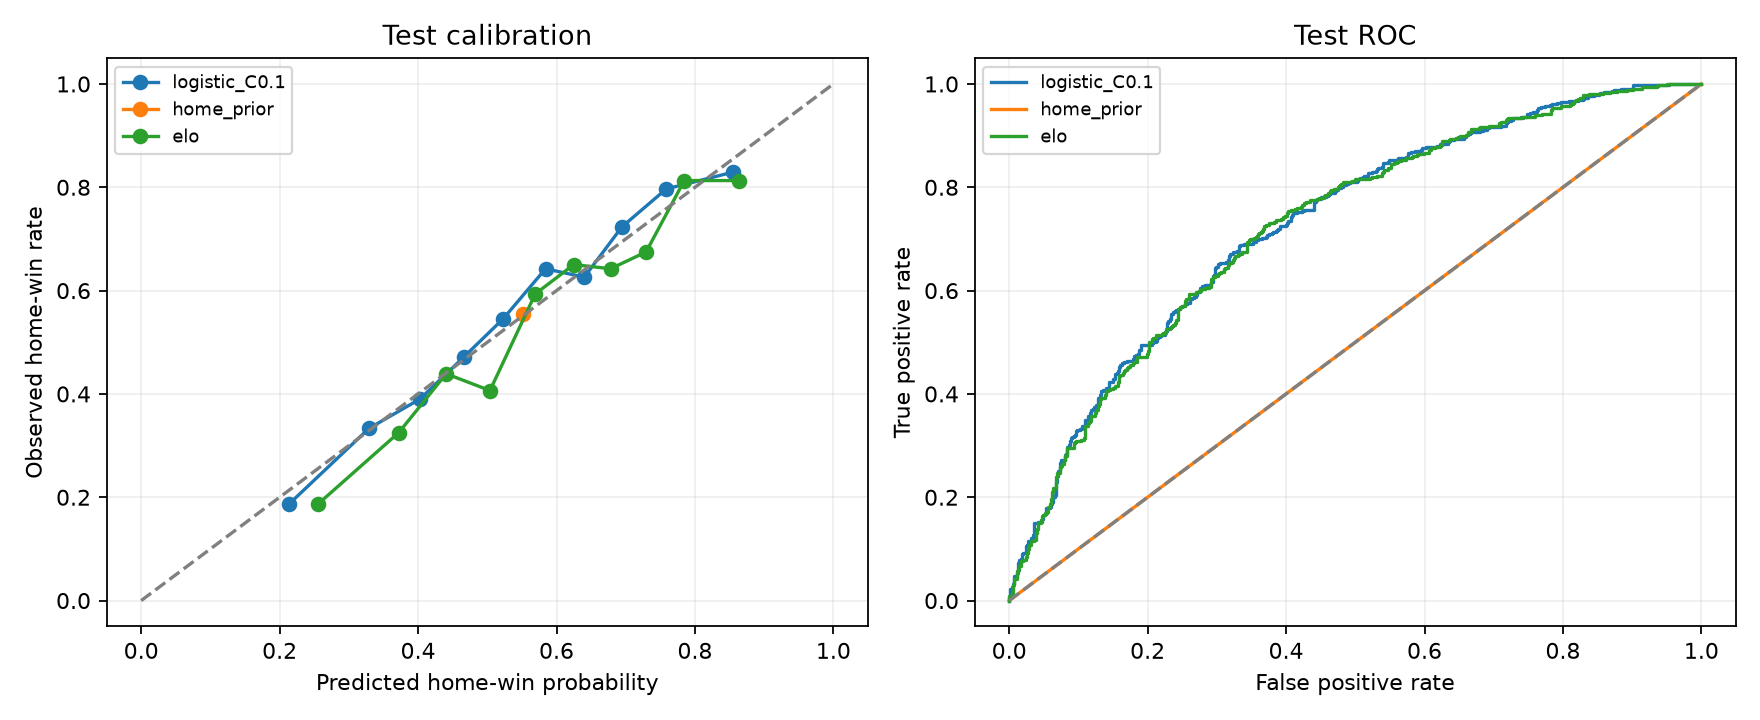
\includegraphics[width=0.92\textwidth]{resultados_calibracao_roc.png}
\caption{Calibração e ROC no teste, reproduzidas do relatório do módulo de previsão de resultados.}
\label{fig:calibracao}
\end{figure*}

A Figura~\ref{fig:calibracao} complementa as métricas agregadas.
A análise de importância por permutação foi realizada na validação,
antes do reajuste final, evitando utilizar o teste para orientar a
seleção das características.

\section{Jogadores e cinco iniciais}

Foi selecionada regressão Ridge com regularização 1 para produção
individual. A Tabela~\ref{tab:producao} compara o MAE com a média das
últimas dez participações e apresenta RMSE e \(R^2\) do modelo.

\begin{table*}[htbp]
\centering
\caption{Erros de teste da produção individual, nas unidades de cada alvo.}
\label{tab:producao}
\begin{tabular}{lrrrr}
\toprule
Alvo & MAE Ridge & MAE média histórica & RMSE Ridge & \(R^2\) Ridge\\
\midrule
Pontos & 4,643 & 4,671 & 6,056 & 0,507\\
Ressaltos & 1,931 & 1,936 & 2,530 & 0,419\\
Assistências & 1,371 & 1,376 & 1,858 & 0,480\\
\bottomrule
\end{tabular}
\end{table*}

As melhorias de MAE são pequenas nos três alvos. Estes resultados
justificam conservar a referência histórica na comparação e não permitem
concluir que o modelo produza uma avaliação geral da qualidade dos jogadores.
A previsão continua condicionada à participação e à existência de histórico.

Para os cinco iniciais foi selecionado o modelo Ridge aditivo, sem
interações de quinteto, com regularização 100. O RMSE de teste foi
15,503 pontos, face a 16,407 da margem média em casa; o MAE foi 12,153 e
\(R^2=0{,}107\). Foram registadas 1\,210 posições de titular ocupadas por
jogadores desconhecidos do modelo no teste. O erro e a variância explicada
mostram que os titulares só capturam uma parte limitada da margem final.
A melhoria sobre a referência não demonstra o efeito causal de escolher
um determinado quinteto ou de realizar uma substituição.

\section{Rotação sujeita a restrições}

O cenário documentado considera Boston em 1 de abril de 2026, como equipa
da casa, com disponibilidade assumida. É um exemplo retrospetivo, sem
certificação do plantel ou da disponibilidade real nessa data.
O solver devolveu \texttt{OPTIMAL}, com utilidade e limite superior de
148,655. A Tabela~\ref{tab:rotacao} apresenta os oito jogadores utilizados;
os restantes candidatos receberam zero minutos.

\begin{table*}[htbp]
\centering
\caption{Rotação registada no cenário autónomo do módulo de planeamento de rotações.}
\label{tab:rotacao}
\begin{tabular}{llr}
\toprule
Jogador & Titular & Minutos\\
\midrule
Derrick White & Sim & 36\\
Jaylen Brown & Sim & 36\\
Jayson Tatum & Sim & 36\\
Sam Hauser & Sim & 28\\
Nikola Vucevic & Sim & 12\\
Neemias Queta & Não & 36\\
Payton Pritchard & Não & 36\\
Baylor Scheierman & Não & 20\\
\midrule
Total & & 240\\
\bottomrule
\end{tabular}
\end{table*}

O relatório regista aprovação nas verificações independentes de posições,
disponibilidade, titulares, minutos e descanso. A optimalidade refere-se
ao problema inteiro formulado, não à melhor decisão desportiva real.
Não foi documentada uma comparação que demonstre ganhos de vitórias
resultantes desta distribuição.

\section{Comparação das políticas de substituição}

No cenário autónomo, as políticas MDP, fixa e gulosa obtiveram a mesma
utilidade esperada exata: 131,7744. Foram avaliadas 500 trajetórias
emparelhadas de contexto e exportados 46 estados de decisão. O ganho
simulado foi zero; não se observou melhoria da política MDP.

As rotações exportadas e simuladas passaram as verificações do módulo de planeamento de rotações
e a preservação exata dos minutos por período. Os orçamentos por período
e os limites de utilização consecutiva restringem as possibilidades de
adaptação. O resultado evidencia a necessidade de avaliar se o espaço de
ações permite diferenças úteis, antes de atribuir vantagens à utilização
de um método sequencial. A utilidade 131,7744 não é diretamente comparável
com 148,655 do módulo de planeamento de rotações, pois as funções objetivo são distintas.

\subsection{Comparação com o algoritmo genético}

O experimento alargado compara políticas adaptativas obtidas pelo AG e
pela programação dinâmica, juntamente com as referências fixa e gulosa.
A Tabela~\ref{tab:genetico} apresenta a utilidade esperada exata no cenário
base e na análise de sensibilidade sem penalização de fadiga.

\begin{table*}[htbp]
\centering
\caption{Utilidade esperada no mesmo MDP para cada cenário de fadiga.}
\label{tab:genetico}
\begin{tabular}{lrr}
\toprule
Política & Cenário base (\(f=0{,}08\)) & Sem penalização (\(f=0\))\\
\midrule
Algoritmo genético & 131,774382 & 140,841917\\
Programação dinâmica exata & 131,774382 & 140,841917\\
Ordem fixa & 131,774382 & 140,829836\\
Política gulosa & 131,774382 & 140,829836\\
\bottomrule
\end{tabular}
\end{table*}

Em ambos os cenários, as cinco execuções genéticas atingem o valor da
solução exata, com diferença nula para o ótimo à precisão reportada.
A execução selecionada usa a semente 42. Cada execução utiliza população
40 e 40 gerações, avaliando os oito cromossomas distintos possíveis.
Apenas três dos 46 estados viáveis têm mais de uma ação, pelo que este
resultado não demonstra vantagem de pesquisa num espaço complexo.

No cenário base, as quatro políticas permanecem equivalentes. Quando se
retira a penalização de fadiga, o AG e a programação dinâmica superam as
referências em cerca de 0,012081 unidades de utilidade esperada. É uma
diferença pequena e dependente da recompensa assumida, não um ganho
medido em pontos ou vitórias. A comparação deve ser feita entre políticas
dentro de cada cenário, pois alterar a penalização também altera a escala
e os valores da recompensa.

Cada comparação utiliza 500 trajetórias emparelhadas e as rotações passam
as verificações de restrições. A Figura~\ref{fig:convergencia-ag} reproduz
a convergência do cenário base. A ausência de melhoria ao longo das gerações
é compatível com um espaço de apenas oito cromossomas e não constitui
prova de convergência rápida em problemas maiores.

\begin{figure*}[htbp]
\centering
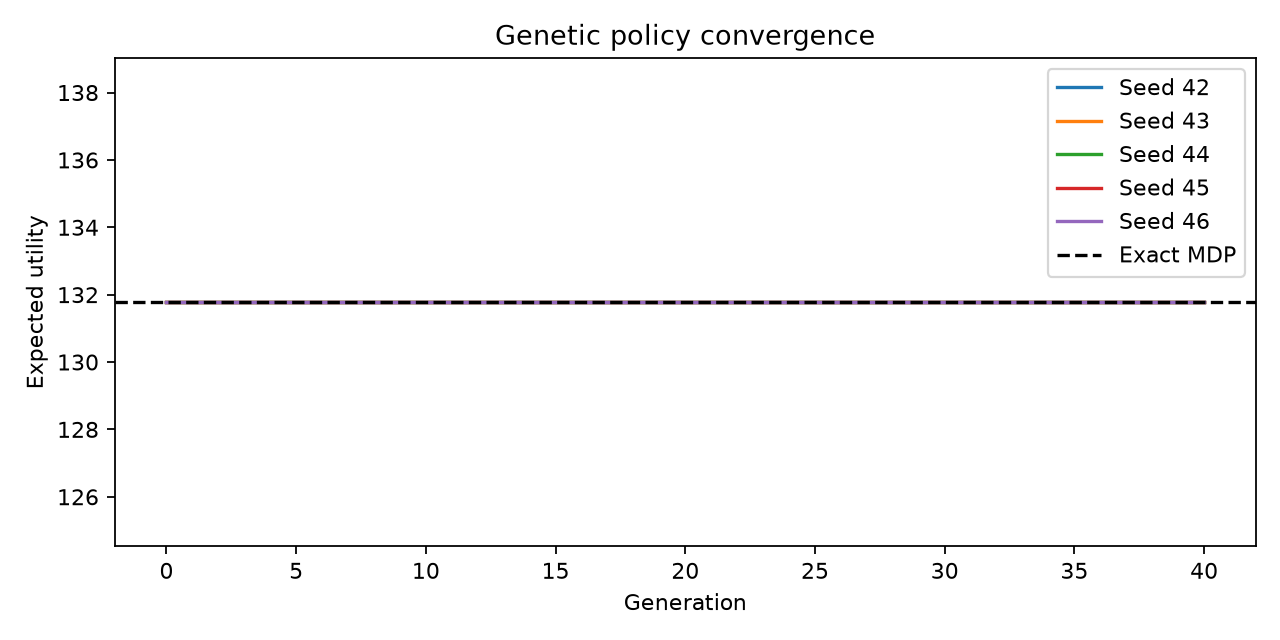
\includegraphics[width=0.85\textwidth]{substituicoes_convergencia_ag.png}
\caption{Convergência genética no cenário base, reproduzida do relatório
 de comparação do módulo de planeamento de substituições.}
\label{fig:convergencia-ag}
\end{figure*}

\section{Horizonte integrado de três jogos}

O cenário integrado usa a data de corte de 1 de abril de 2026 e os três
jogos seguintes registados para Boston. O objetivo é atingir pelo menos
duas vitórias. O relatório apresenta 2,062 vitórias esperadas e
probabilidade de 77,1\% de cumprir o objetivo, sob independência dos
resultados. A Tabela~\ref{tab:horizonte} resume as previsões e a seleção.

\begin{table*}[htbp]
\centering
\caption{Plano integrado, com informação congelada antes da data de corte.}
\label{tab:horizonte}
\begin{tabular}{lrr}
\toprule
Data & Probabilidade de vitória & Limite do candidato selecionado\\
\midrule
1 de abril de 2026 & 59,5\% & 32 minutos\\
3 de abril de 2026 & 78,4\% & 32 minutos\\
5 de abril de 2026 & 68,3\% & 32 minutos\\
\bottomrule
\end{tabular}
\end{table*}

A seleção foi \texttt{OPTIMAL} entre os candidatos gerados, respeitando o
limite de 96 minutos por jogador no horizonte. O limite de 64 minutos em
dias consecutivos está configurado, mas não é exercitado por estas três
datas, separadas por dois dias. A probabilidade de cumprir o objetivo é
calculada a partir das previsões, não de um efeito das rotações selecionadas.

\section{Limitações e alcance da avaliação}

Os resultados de aprendizagem descrevem uma única divisão temporal.
Faltam avaliações em temporadas alternativas e estimativas da incerteza
das diferenças preditivas. As lacunas das fontes, a exclusão de lesões,
os registos retrospetivos de titulares e as posições sem histórico
condicionam a interpretação.

No planeamento, os pesos de utilidade, a fadiga, os contextos e as transições
são hipóteses explícitas. A integração demonstra compatibilidade entre
módulos e cumprimento de restrições nos cenários documentados, mas não
valida essas hipóteses nem demonstra superioridade de decisões em jogos
reais. Seriam necessárias comparações adicionais, com diferentes plantéis,
calendários, indisponibilidades e orçamentos, para avaliar a generalização.
